% Copy this package's output/ and captions.tex next to this snippet, or
% adjust paths. Choose the main-text version before editing the manuscript.
% Verified captions. The caller needs graphicx and amsmath.
\newcommand{\OverviewCaption}[1]{Representative #1 fields across three flow benchmarks.
Columns show the POD-reconstructed reference, the case-specific prediction,
and pointwise absolute error. Circular uses the original-initialization
Periodic sparse-MoE specialist (seed 1248); Square uses T2-C with fixed
sparse-MoE candidates; Pinball uses T2-C with Deep-FNN-H3 candidates.
The first archived valid window at the lowest held-out Reynolds number is
shown at its endpoint: Circular, window 976, $t_0=1384.4960$,
$\Delta T=598.7009$, $K=48$; Square H--P, window 506, $t_0=8$,
$\Delta T=96$, $K=24$; Pinball H--P, window 2, $t_0=36.75$,
$\Delta T=14$, $K=56$.
Velocity panels show $\|\mathbf{u}\|_2$ and errors
$\|\mathbf{u}_{\rm pred}-\mathbf{u}_{\rm ref}\|_2$;
pressure panels show weighted-zero-mean kinematic pressure $p^\circ$
and $|p^\circ_{\rm pred}-p^\circ_{\rm ref}|$.
Coordinates, time, and fields retain their native dataset scales; no
additional cross-case nondimensionalization is imposed. In particular,
the Circular source uses fixed $\nu=0.001$.
Each row uses a joint full-domain field range and a separate zero-based
error range, without percentile clipping. The color scales are
case-specific and support within-row comparison only. These snapshots
are neither a matched architecture ablation nor evidence of one model's
zero-shot transfer between geometries.}

\newcommand{\FusionCaption}[2]{Frozen output-space fusion on held-out #1
windows, displaying #2. Each case block shows the POD reference,
the actual frozen E2 Top-1 prediction, and T2-C, followed by their
two pointwise error fields. E2 is obtained by the global three-class
router argmax; it selects a member of the prescribed pair in all shown
windows, without using test errors. Square uses archived sparse-MoE
candidates; Pinball uses Deep-FNN-H3 candidates. The displayed T2-C
weight multiplies the first named candidate and is fixed from the
initial history throughout the rollout; there is no fusion feedback.
Velocity error is $\|\mathbf{u}_{\rm pred}-\mathbf{u}_{\rm ref}\|_2$;
pressure error is $|p^\circ_{\rm pred}-p^\circ_{\rm ref}|$ after the
same quadrature-weighted zero-mean gauge. All fields retain native
dataset scales. Within each case, the three physical fields share
one full-range scale and the two errors share one zero-based scale,
with no clipping or smoothing. Case-specific scales are not comparable
across rows. The first common valid window at the lowest held-out Re
is shown at its endpoint, not selected by fusion benefit.}

\newcommand{\HPWindows}{Square: window 506, $t_0=8$, $\Delta t=4$,
$K=24$, $t=104$. Pinball: window 2, $t_0=36.75$,
$\Delta t=0.25$, $K=56$, $t=50.75$. Circular is not included in this
H--P comparison because a matching verified H--P fusion field set
was not established.}
\newcommand{\SHWindows}{Square: window 7814, $t_0=8$, $\Delta t=4$,
$K=24$, $t=104$. Pinball: window 514, $t_0=0.75$,
$\Delta t=0.25$, $K=56$, $t=14.75$. This supplement covers these two
verified cases only; it is not a claim that Circular S--H fusion data
do not exist.}

\begin{figure}[t]
  \centering
  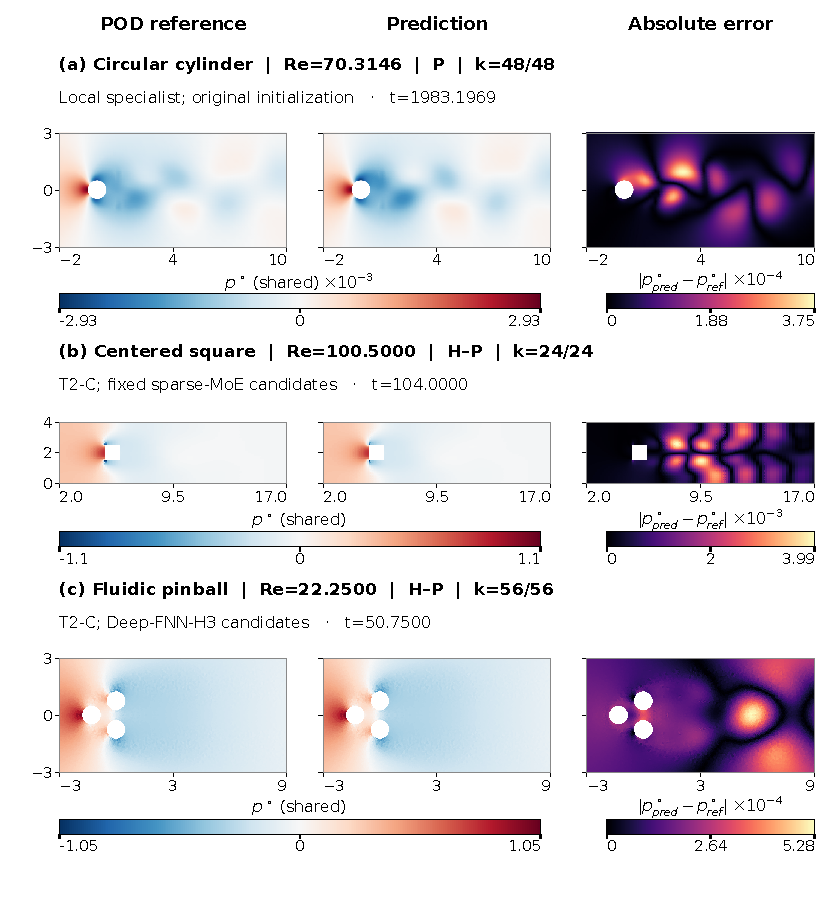
\includegraphics[width=\linewidth]{output/field_overview_three_cases_pressure.pdf}
  \caption{\OverviewCaption{pressure}}
  \label{fig:field-overview-pressure}
\end{figure}

\begin{figure}[t]
  \centering
  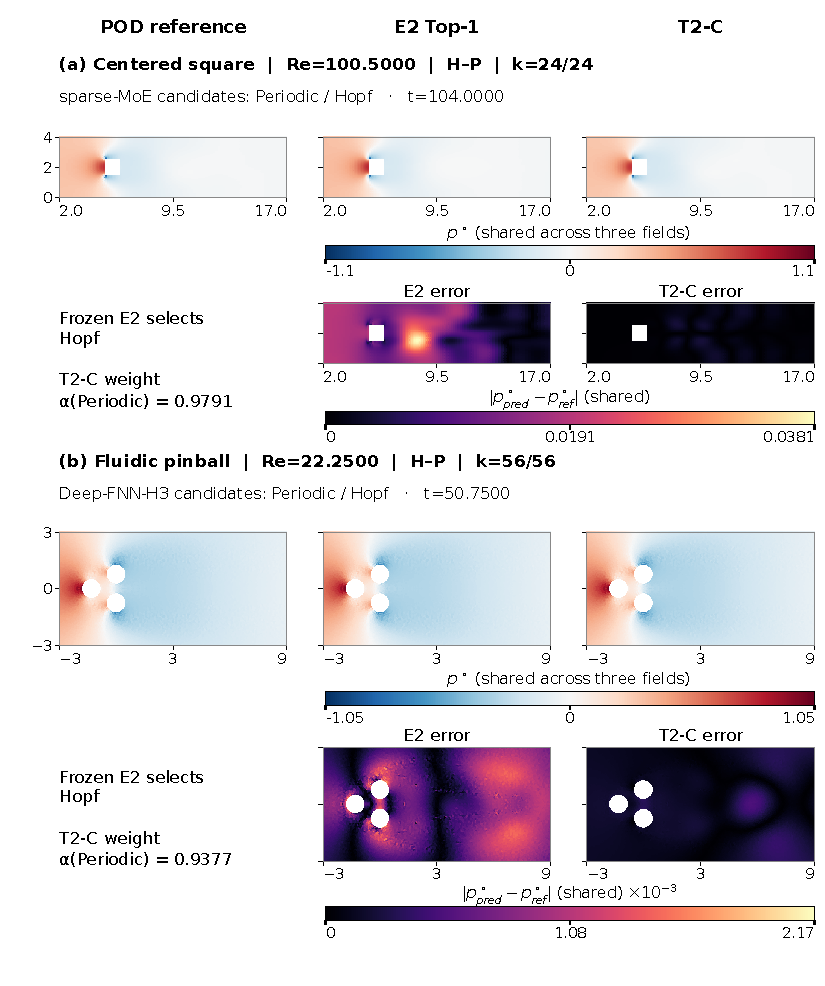
\includegraphics[width=\linewidth]{output/fusion_comparison_hp_square_pinball_pressure.pdf}
  \caption{\FusionCaption{H--P}{pressure} \HPWindows}
  \label{fig:fusion-hp-verified-pressure}
\end{figure}
% Alternatives: replace pressure with velocity in the filename and caption.
% S--H supplement: fusion_comparison_sh_square_pinball_pressure.pdf,
% with \FusionCaption{S--H}{pressure} \SHWindows.
